\documentclass[aspectratio=169]{beamer}
\usetheme{metropolis}  

\metroset{block=fill}

\setlength{\parindent}{0pt}
\usepackage[utf8]{inputenc}
\usepackage{amsbsy}
\usepackage{amsmath}
\usepackage{enumitem}
\usepackage{hyperref}
\usepackage{array}
\usepackage[T1]{fontenc}
\usepackage{tikz}
\usepackage{latexsym,xcolor,multicol,booktabs,calligra}
\usepackage{amsmath,amssymb,BOONDOX-cal,bm}	
\usepackage{graphicx,stackengine}   
\usepackage{xcolor}
\usepackage[sfdefault]{AlegreyaSans}
\usepackage{tabularx} 

\definecolor{white}{RGB}{255,255,255}
\setbeamercolor{background canvas}{bg=white}
\setbeamercolor{normal text}{bg=white}

\title{Causal Inference Project:\\ Impact of Scholarships on Student Success}
\date{April 04th, 2025}
\author{Anushka Mukherjee, Lucie Marimar, Jort Koks, Jakob Sarrazin}
\institute{Machine Learning for Econometrics \\ ENSAE, IP Paris \\ Bruno Crépon, Matthieu Doutreligne}

% ---------------------------------------
% Begin Document
% ---------------------------------------

\begin{document}
  \maketitle
  
   \section{1. Motivation}
  
  \begin{frame}{Motivation I}
  		\begin{columns}
	\begin{column}{0.7\textwidth}
	\textbf{Retention and Completion: A Core Challenge for Universities}

  		\begin{itemize}
  		\item [$\rightarrow$] \textbf{High dropout rates} are a persistent issue in higher education, especially during the first years of study.
  		\item [$\rightarrow$] \textbf{Timely graduation} is crucial for both students (career entry) and universities (funding, reputation
  		\item [$\Rightarrow$] \textbf{Financial constraints} are a major barrier to academic success — especially for socio-economically disadvantaged students.
  	\end{itemize}
  \end{column}

	\begin{column}{0.3\textwidth}
	\begin{center}
     \includegraphics[width=1\textwidth]{Tex_Pictures/Hat.jpg}
     \end{center}
	\end{column}

\end{columns}

  	
  \end{frame}
  
  \begin{frame}{Motivation II}
  	\textbf{Scholarships as a Tool to Improve Student Retention and Graduation}
  	
  	\begin{itemize}
  		\item [$\rightarrow$]  \textbf{Scholarship programs} are widely used as an intervention, but:
  		\begin{itemize}
  		  		\item [--] Their  \textbf{causal effect} on student outcomes is difficult to measure
  		  		\item [--] Many studies show correlations, but few rigorously identify causality.
   		\end{itemize}
   		\item [$\rightarrow$] This study uses a \textbf{causal machine learning framework (DML)} to estimate the  \textbf{true effect of scholarships}, adjusting for observed confounders.
   		\item [$\rightarrow$] Findings can inform \textbf{policy decisions} on financial aid allocation and \textbf{targeting of support} for at-risk students.
  	\end{itemize}
  \end{frame}
  
  \section{2. PICO \& Research Question}
  
  \begin{frame}{PICO Formulation}
  \textbf{Population, Intervention, Comparison, Outcome}
  	\begin{itemize}
  		\item [P - ] Undergraduate students at a Portuguese university (N = 4,424), with data on demographics, socio-economic background, and prior academic performance.
  		\item [I - ] Receiving a scholarship during university studies.
  		\item [C - ] Students without scholarships, adjusted for observed confounders (grades, family background, gender, etc.).
  		\item [O - ] Two binary outcomes observed 3 years after enrollment:
  
  	\begin{itemize}
  		\item [1.] Dropout vs. Enrolled/Graduated
  		\item [2.] Graduated vs. Dropout/Enrolled
  	\end{itemize}
  	
  	\end{itemize}
  \end{frame}

  
  \begin{frame}{Research Question}
    \begin{alertblock}{RQ1}
	Does receiving a scholarship \textbf{reduce} the likelihood of \textbf{dropping out} within 3 years?
\end{alertblock}
\vspace{10pt}
    \begin{alertblock}{RQ2}
	Does receiving a scholarship \textbf{increase} the likelihood of \textbf{graduating} within 3 years?
\end{alertblock}
  \end{frame}
  

\section{3. Data Overview and Exploratory Analysis}

\begin{frame}{The Data}
	\textbf{Source}
	\begin{itemize}
		\item [--] UCI Machine Learning Repository – Predict Students Dropout and Academic Success 
	\end{itemize}
	
	\textbf{Scope}
	\begin{itemize}
		\item [--] Administrative records from a Portuguese university $\rightarrow$ 4,424 undergraduate students across various degree programs
	\end{itemize}
	
	\textbf{Observation Period}
	\begin{itemize}
		\item [--] Students tracked for 3 years after enrollment.
	\end{itemize}
\end{frame}

\begin{frame}{Variables}
\centering
\renewcommand{\arraystretch}{1.4}

\begin{tabularx}{\textwidth}{X | X | X}
\textbf{Outcome Variable} & \textbf{Treatment Variable} & \textbf{Covariates}  (Pre Treatment)\\[0.5ex]
\hline \hline 
Student status after 3 years: 
\parbox[t]{4cm}{\vspace{-12pt} \begin{itemize}[label=--,leftmargin=1.2em,itemsep=1pt,topsep=2pt]
    \item Dropout
    \item Still enrolled
    \item Graduated
    \item[$\rightarrow$] \textit{Re-coded into two binary variables for RQ1 \& RQ2}
\end{itemize}} &

Received scholarship or not (\textit{Binary variable}) 

& \vspace{-27pt}
\parbox[t]{4cm}{\begin{itemize}[label=--,leftmargin=1.2em,itemsep=1pt,topsep=2pt]
    \item Academic performance before university
    \item Family background
    \item Economic context
    \item Demographics
\end{itemize}}

\end{tabularx}
\end{frame}

\begin{frame}{Outcome Variable}
	\begin{center}
     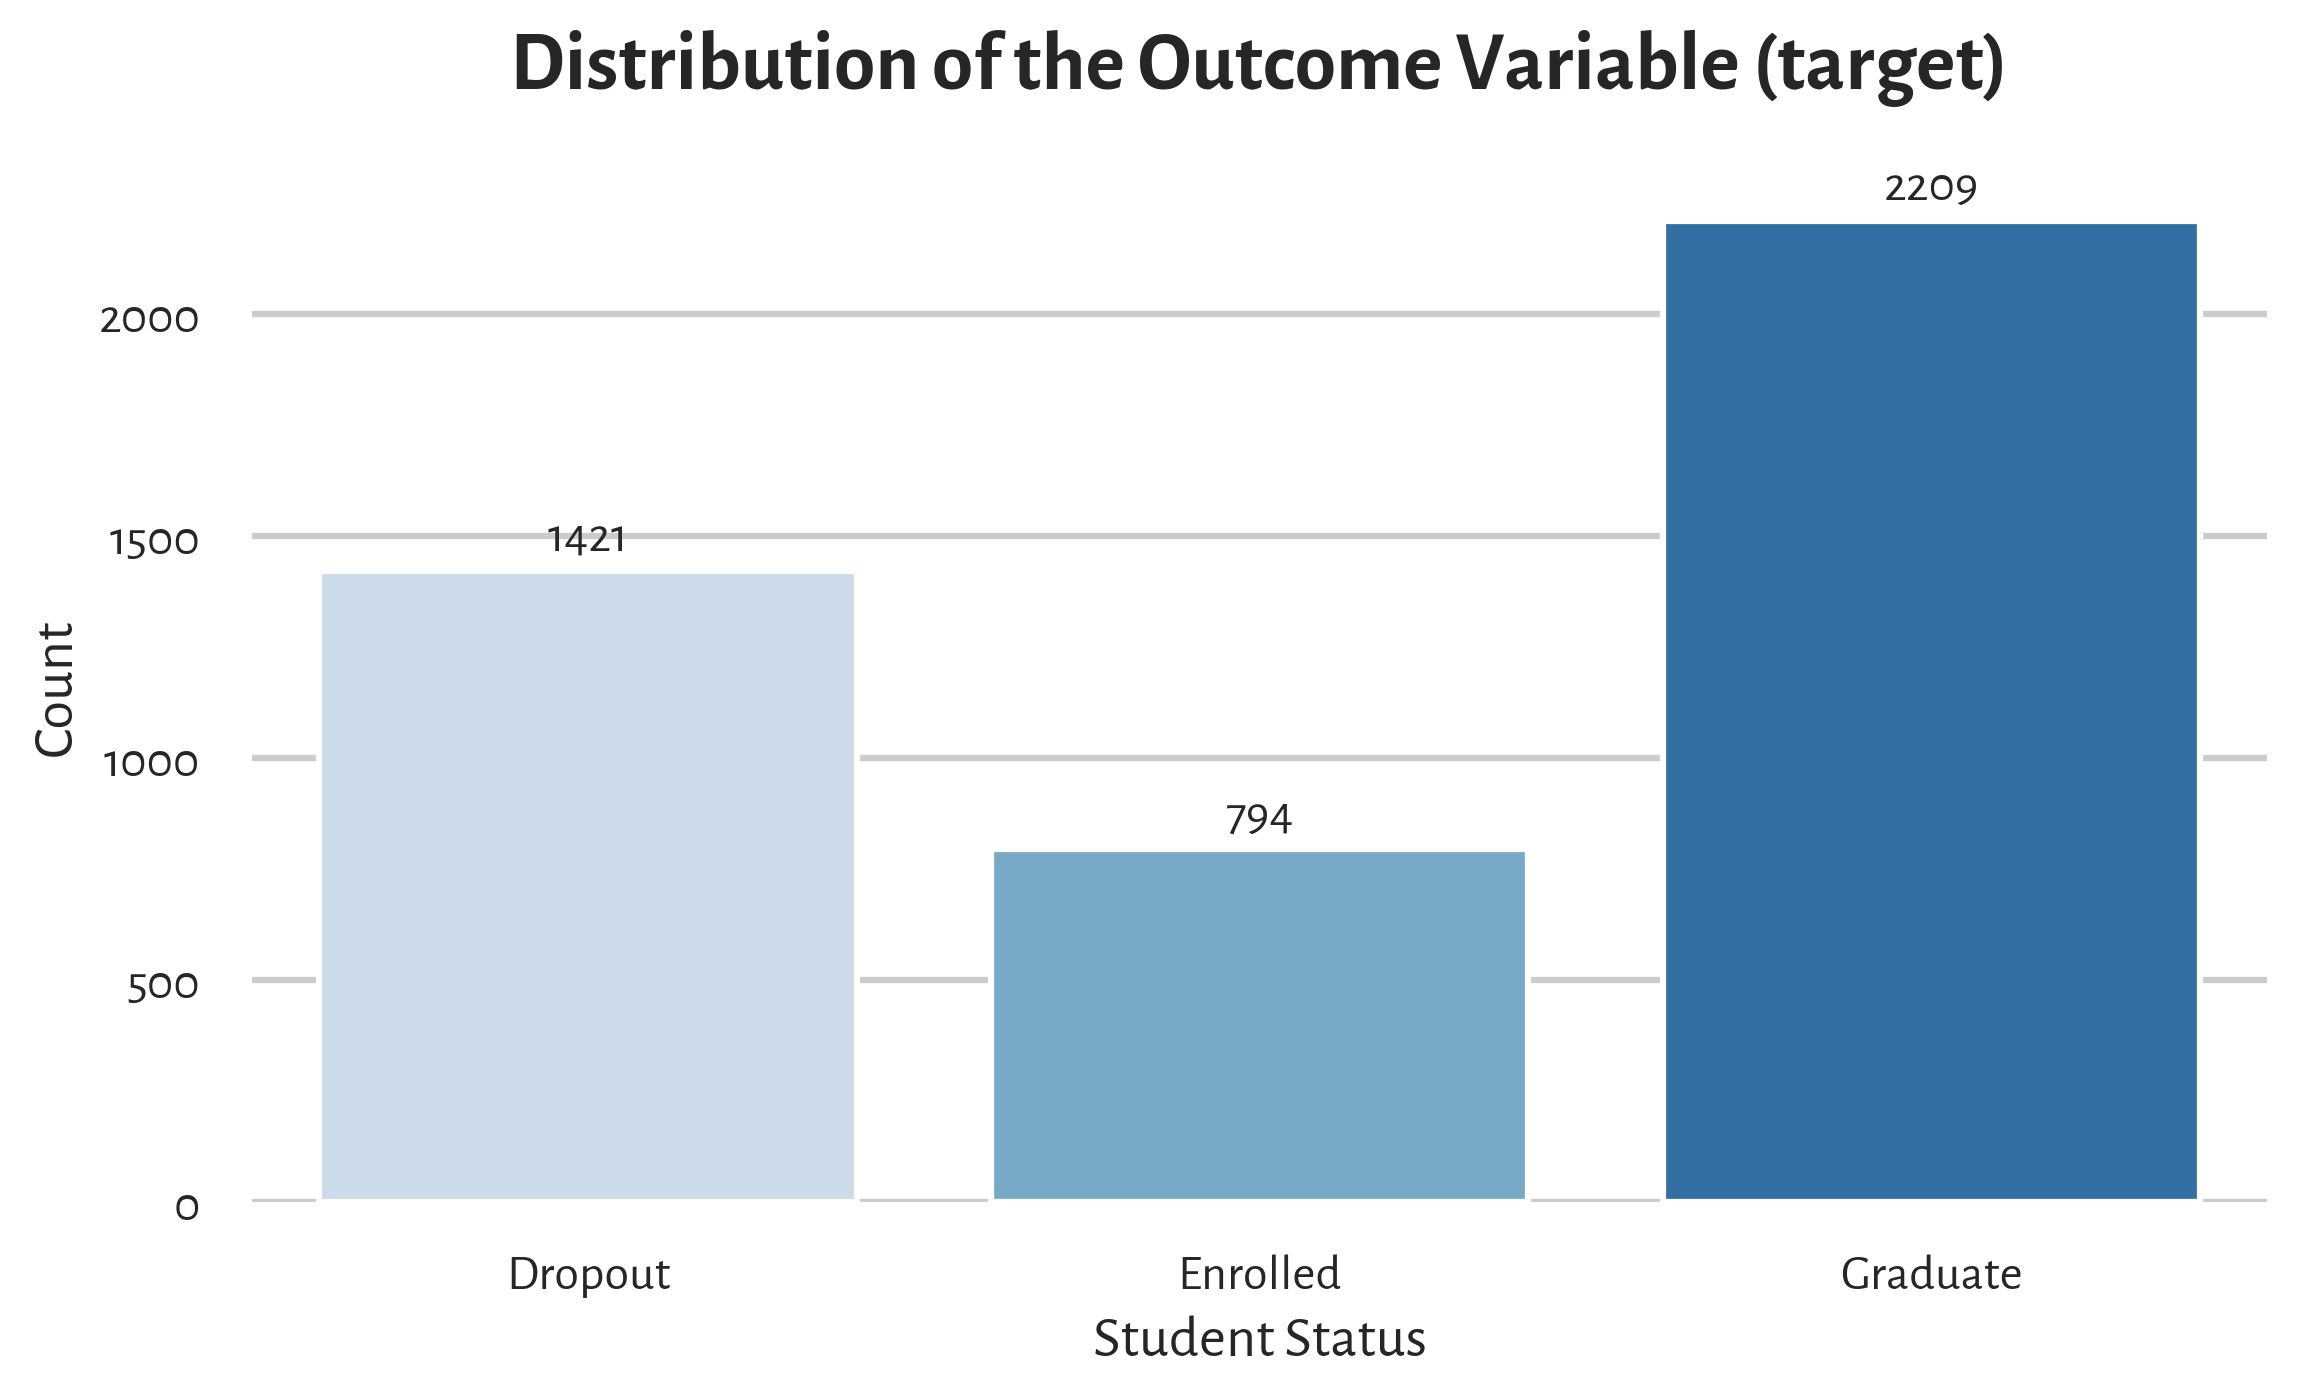
\includegraphics[width=0.85\textwidth]{Tex_Pictures/Graph1.png}
     \end{center}
\end{frame}

\begin{frame}{Treatment vs Outcome Variable}
	\begin{center}
     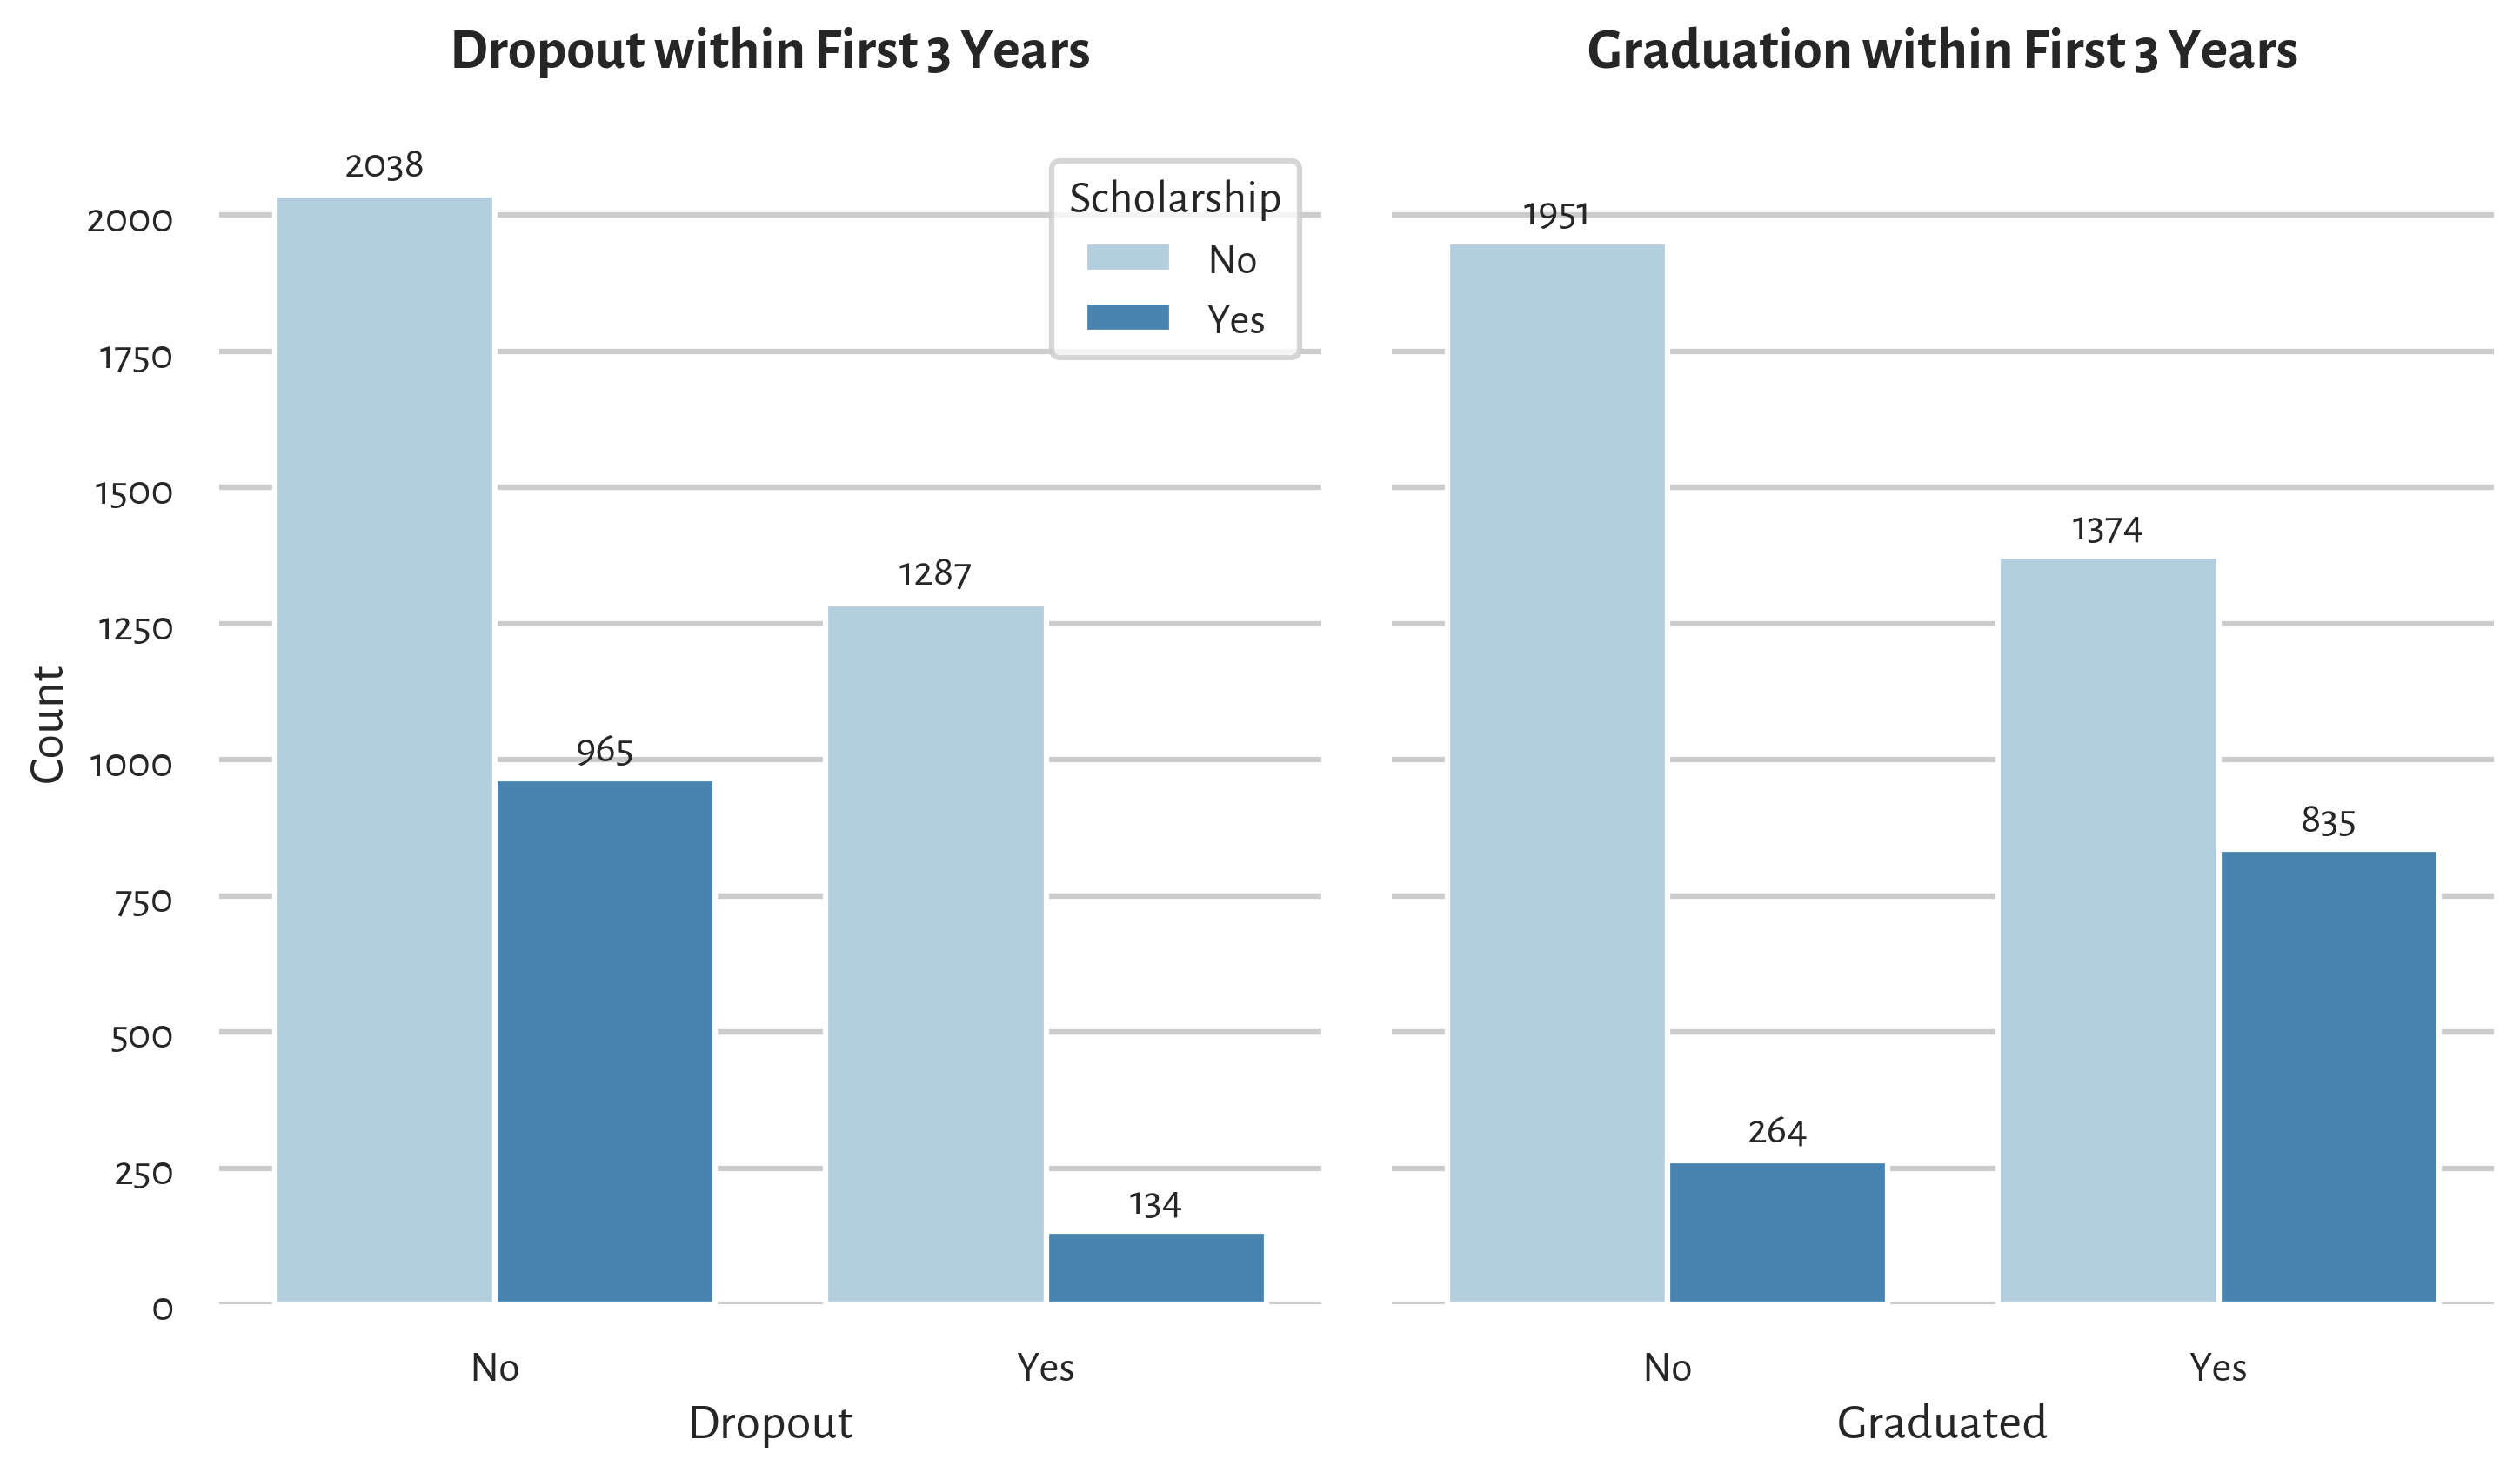
\includegraphics[width=0.9\textwidth]{Tex_Pictures/Graph2.png}
     \end{center}
\end{frame}

\begin{frame}{Covariates}
	
\end{frame}

\section{4. Causal Graph and Covariate Selection}

\section{5. Causal Effect Estimation Using Double Post Lasso}

\section{6. Causal Effect Estimation Using Double Machine Learning}


\section{X. Conclusion}

  
\end{document}